\iffalse

\documentclass[handout]{mcs}

\begin{document}

\formatpages{}{Appendix, Class Problems 7F}{Fri, October 23}
\fi

\section*{Appendix}

\begin{definition}
  A \term{planar embedding} of a \term{connected} graph consists of a
  nonempty set of cycles of the graph called the \term{discrete faces}
  of the embedding.  Planar embeddings are defined recursively as
  follows:

\begin{itemize}
\item \textbf{Base case:} If $G$ is a graph consisting of a single vertex,
$v$, then a planar embedding of $G$ has one discrete face, namely the
length zero cycle, $v$.

\item \textbf{Constructor Case:} (split a face) Suppose $G$ is a
connected graph with a planar embedding, and suppose $a$ and $b$ are
distinct, nonadjacent vertices of $G$ that appear on some discrete face,
$\gamma$, of the planar embedding.  That is, $\gamma$ is a cycle of the form
\[
a \dots b \cdots a.
\]
Then the graph obtained by adding the edge $\edge{a}{b}$ to the edges of
$G$ has a planar embedding with the same discrete faces as $G$, except
that face $\gamma$ is replaced by the two discrete
faces\footnote{\label{cp7f.C} There is one exception to this rule.  If $G$ is a
line graph beginning with $a$ and ending with $b$, then the cycles into
which $\gamma$ splits are actually the same.  That's because adding edge
$\edge{a}{b}$ creates a simple cycle graph, $C_n$, that divides the plane
into an ``inner'' and an ``outer'' region with the same border.  In order
to maintain the correspondence between continuous faces and discrete
faces, we have to allow two ``copies'' of this same cycle to count as
discrete faces.  But since this is the only situation in which two faces
are actually the same cycle, this exception is better explained in a
footnote than mentioned explicitly in the definition.}
\[
a\dots ba\quad \text{ and } ab\cdots a, 
\]
as illustrated in Figure~\ref{cp7f.fig:face-splitting}.

\begin{figure}[h]
\centering 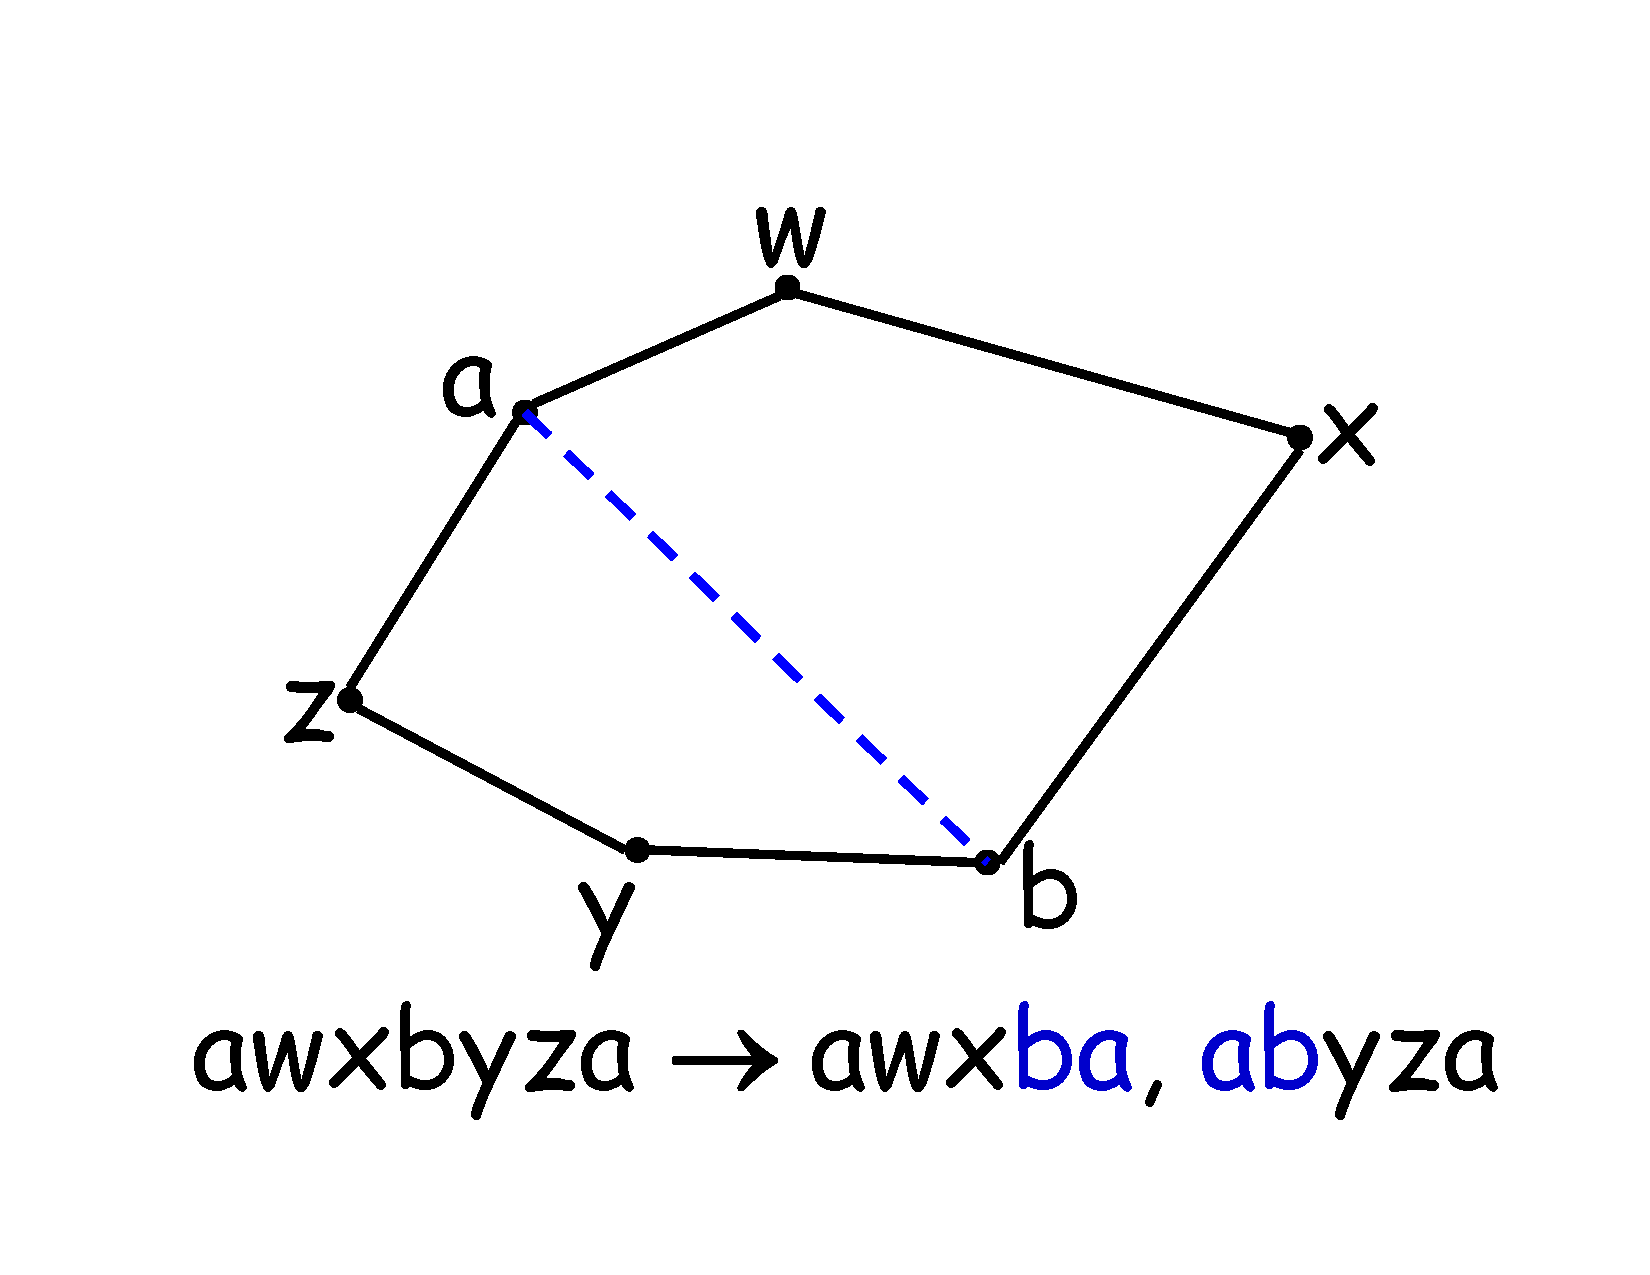
\includegraphics[height=2.5in]{figures/split-a-face}
\caption{The Split a Face Case.}
\label{cp7f.fig:face-splitting}
\end{figure}

\item \textbf{Constructor Case:} (add a bridge) Suppose $G$ and $H$ are
connected graphs with planar embeddings and disjoint sets of vertices.
Let $a$ be a vertex on a discrete face, $\gamma$, in the embedding of
$G$.  That is, $\gamma$ is of the form
\[
a\dots a.
\]
Similarly, let $b$ be a vertex on a discrete face, $\delta$, in the
embedding of $H$, so $\delta$ is of the form
\[
b\cdots b.
\]
Then the graph obtained by connecting $G$ and $H$ with a new edge,
$\edge{a}{b}$, has a planar embedding whose discrete faces are the union of
the discrete faces of $G$ and $H$, except that faces $\gamma$ and $\delta$
are replaced by one new face
\[
a\dots ab\cdots ba,
\]
as illustrated in Figure~\ref{cp7f.fig:add-bridge}.

\begin{figure}[h]
\centering 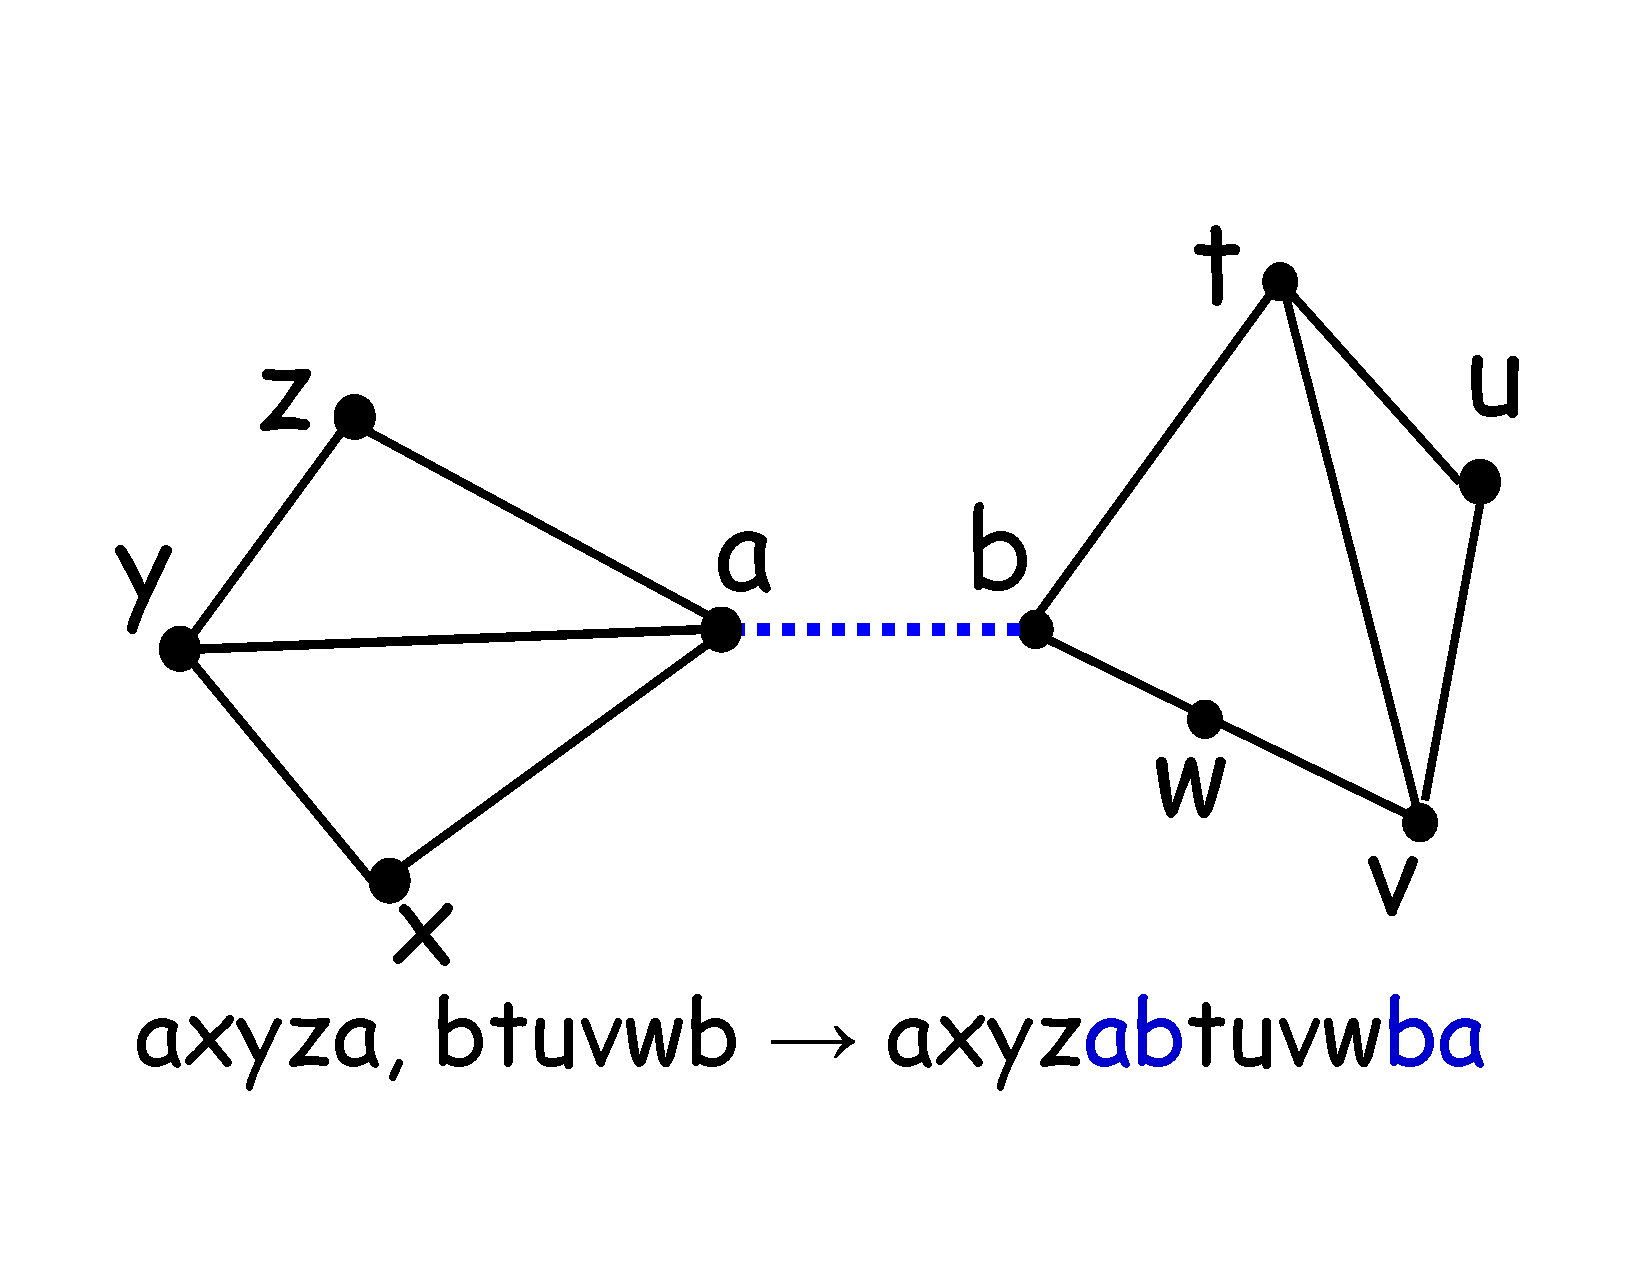
\includegraphics[height=3in]{figures/add-bridge}
\caption{The Add Bridge Case.}
\label{cp7f.fig:add-bridge}
\end{figure}

\end{itemize}

An arbitrary graph is \term{planar} iff each of its connected
components has a planar embedding.

\end{definition}

%\instatements{\newpage}
\begin{theorem}[Euler's Formula]
If a connected graph has a planar embedding, then
%
\[
v - e + f = 2
\]
%
where $v$ is the number of vertices, $e$ is the number of edges, and
$f$ is the number of faces.
\end{theorem}

\begin{corollary}
\label{cp7f.3v}
Suppose a connected planar graph has $v \geq 3$ vertices and $e$ edges.  Then
\[
e \leq 3v-6.
\]
\end{corollary}

\begin{proof}
By definition, a connected graph is planar iff it has a planar embedding.
So suppose a connected graph with $v$ vertices and $e$ edges has a planar
embedding with $f$ faces.  By
Problem~\ref{planar-structural}.\ref{structind-twice}, every edge is traversed
exactly twice by the face boundaries.  So the sum of the lengths of the
face boundaries is exactly $2e$.  Also by
Problem~\ref{planar-structural}.\ref{structind-face-length}, when $v \geq 3$, each
face boundary is of length at least three, so this sum is at least $3f$.
This implies that
\begin{equation}\label{cp7f.e3f}
3f \leq 2e.
\end{equation}
But $f = e-v+2$ by Euler's formula, and substituting into~\eqref{cp7f.e3f} gives
\begin{align*}
3(e-v+2) & \leq 2e\\
e-3v + 6  & \leq 0\\
e & \leq 3v - 6
\end{align*}
\end{proof}

\begin{corollary}
$K_5$ is not planar.
\end{corollary}

\begin{proof}
\[
e = 10 > 9 = 3v-6.
\]
\end{proof}
\iffalse

\end{document}
\fi

\endinput
